    \documentclass[12pt]{article}
    \usepackage[utf8]{inputenc}
    \usepackage{polski}
    \usepackage{enumitem}
    \usepackage{newunicodechar}
    \usepackage{amsmath}
    \usepackage{tikz}

    \newcommand{\floor}[1]{\left\lfloor #1 \right\rfloor}
    \setcounter{MaxMatrixCols}{20}

    \title{Zadanie 6}
    \author{Patryk Lisik}
    \date{\(11\) Lutego  2024}

    \begin{document}

    \maketitle
    \renewcommand{\abstractname}{Treść}

    \begin{abstract}
    Dla kodera spoltowego wyznacz wielomian generujący i zakoduj wiadomość $\mathbf{m} = (101) $ 
    \begin{figure}[h]
        \centering
        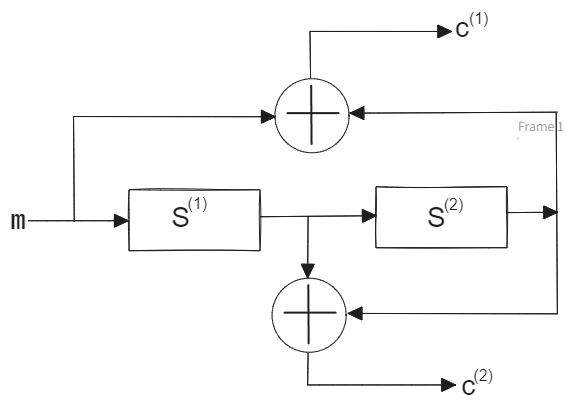
\includegraphics[width=8cm]{cyclic_koder.png}
    \end{figure}

    % \begin{tikzpicture}
        %     \filldraw[black] (0,0) circle (2pt) node[anchor=west] (1,2){m};
        %     \draw (1,2) rectangle (4,0);
        %     % \draw (8,1) rectangle (10,2);
        %    
        % \end{tikzpicture}
    \end{abstract}



    \section*{Rozwiązanie}
    \begin{align*}
        S_1(0) = 0 & \\ 
        S_2(0) = 0 & \\
    \end{align*}
    \begin{align*}
        & S_1(t+1)=m(t) & & C_2(t) = m(t) \oplus S_2(t) & & S_1(t)=m(t-1) \\
        & S_2(t+1)=S^{(1)}(t) & & C_2(t) = S_1(t) \oplus S_2(t) & & S_2(t)=m(t-2) \\
    \end{align*}


    \begin{table}[h]
       \centering 
        \begin{tabular}{cccccc}
            i & $m_1$ & $S_i^{(1)}$ & $S_i^{(2)}$ & $C_i^{(1)}$ & $C_i^{(2)}$  \\ \hline
            0 &  1    &  0          &   0         &  1          &  0  \\        
            1 &  0    &  1          &   0         &  0          &  1  \\  
            2 &  1    &  0          &   1         &  0          &  1  \\  
            3 &  0    &  1          &   0         &  0          &  1  \\  
            4 &  0    &  0          &   1         &  1          &  1  \\  
            5 &  0    &  0          &   0         &  0          &  0  \\   
        \end{tabular}
    \end{table}

    \begin{align*}
        & C^{(1)}(D) = M(D)G^{(1)}(D) \\ 
        & C^{(2)}(D) = M(D)G^{(2)}(D) \\ 
        & \begin{pmatrix}
            C^{(1)}(D) \\
            C^{(2)}(D) \\
        \end{pmatrix} = 
        M(D)\begin{pmatrix}
            1 \oplus D^2 \\
            D \oplus D^2 \\
        \end{pmatrix} \\
        & \begin{pmatrix}
            C^{(1)}(D) \\
            C^{(2)}(D) \\
        \end{pmatrix} =
        (1 \oplus D^2)
        \begin{pmatrix}
        1\oplus D^2 \\  
        D \oplus D^2 \\ 
        \end{pmatrix}=\\   
        & = \begin{pmatrix}
            (1\oplus D^2)(1\oplus D^2) \\
            (1 \oplus D^2)(D \oplus D^2) 
        \end{pmatrix} = 
        \begin{pmatrix}
            1\oplus D^2 \oplus D^2 \oplus D^4 \\
            D \oplus D^2 \oplus D^3 \oplus D^4
        \end{pmatrix} = 
        \begin{pmatrix}
            1 \oplus D^4 \\
            D \oplus D^2 \oplus D^3 \oplus D^4
        \end{pmatrix}
    \end{align*}
    
    \begin{multline*}
    C(D) = C^{(1)}(D^2) \oplus DC^{(2)}(D^2) = 1\oplus D^8 \oplus D^3 \oplus D^5 \oplus D^7 \oplus D^9 = \\
    = 1 \oplus D^3 \oplus D^5 \oplus D^7 \oplus D^8 \oplus D^9 
    \end{multline*}

    Finalnie 
    $$c = (100101011) $$

    \end{document}
